\documentclass[10.8pt,fleqn]{report}

\setcounter{tocdepth}{3}
\setcounter{secnumdepth}{3}

\usepackage{a4}
\usepackage{latexsym}
\usepackage{epsf}
\usepackage{listings}
\usepackage{xcolor}
\usepackage{titlesec}
\usepackage{lipsum}
\usepackage{scrextend}
\usepackage{tikz}
\usetikzlibrary{fit}
\usetikzlibrary{calc}
\usetikzlibrary{positioning}
\usetikzlibrary{shadows}
\usetikzlibrary{shadows.blur}
\usetikzlibrary{shapes.symbols}
\usepackage{fontspec}
\usepackage{wrapfig}
\usepackage{nameref}
\usepackage{hyperref}
\usepackage{enumitem}
\usepackage{relsize}
\usepackage{pdfpages}
\usepackage{makeidx}
\usepackage{csquotes}

\usepackage{amsmath, amsthm, amssymb}
\usepackage[ngerman, english]{babel}
\usepackage{marvosym}
\usepackage{graphics}
\usepackage{extarrows}
\usepackage{forloop}
\usepackage{mathtools}

\usepackage[]{algorithm2e}

\usepackage{hyperref}% http://ctan.org/pkg/hyperref
\usepackage{cleveref}% http://ctan.org/pkg/cleveref
\usepackage{lipsum}% http://ctan.org/pkg/lipsum
\newtheorem{definition}{Definition}
\newtheorem{theorem}{Theorem}
\newtheorem{lemma}{Lemma}
\newtheorem{preliminary}{Preliminary}
\newtheorem{notation}{Notation}
\newtheorem{property}{Property}
\newtheorem{corollary}{Corollary}
\newtheorem{example}{Example}
\newtheorem{hypothesis}{Hypothesis}

\usepackage{graphicx}
\usepackage{subfig}

\crefname{theorem}{Theorem}{Theorems}
\crefname{definition}{Definition}{Definitions}
\crefname{lemma}{Lemma}{Lemmas}
\crefname{preliminary}{Preliminary}{Preliminaries}
\crefname{notation}{Notation}{Notations}
\crefname{property}{Property}{Properties}
\crefname{corollary}{Corollary}{Corollaries}
\crefname{example}{Example}{Examples}
\crefname{hypothesis}{Hypothesis}{Hypotheses}


\newenvironment{beweis}{\begin{proof}[Beweis]}{\end{proof}}


\usepackage[font=footnotesize,labelfont=bf]{caption}

\newfontfamily\sansfont[Extension = .ttf, Path = ./fonts/, UprightFont = OpenSans-Regular, BoldFont=OpenSans-SemiBold, ItalicFont=OpenSans-SemiBold]{OpenSans}


\titleformat{\chapter}[display]
  {\sansfont\bfseries}{}{0pt}{\huge}
  
\renewcommand{\contentsname}{\sansfont Content}  

\definecolor{folderbg}{RGB}{70, 130, 180}
\definecolor{folderborder}{RGB}{50,50,50}
\definecolor{DarkGreen}{RGB}{0, 136, 0}
\newlength\Size
\setlength\Size{5pt}


\pgfdeclarelayer{bg}
\pgfsetlayers{bg,main}

\renewcommand{\textfraction}{0.05}
\topmargin -15mm
\textwidth 160mm
\textheight 240mm
\oddsidemargin -2mm
\evensidemargin -2mm

\newcommand\blfootnote[1]{%
  \begingroup
  \renewcommand\thefootnote{}\footnote{#1}%
  \addtocounter{footnote}{-1}%
  \endgroup
}


\usepackage[backend=biber,bibencoding=utf8,style=numeric,autocite=plain,sorting=none]{biblatex}
\usepackage{setspace}

\addbibresource{Literatur.bib}

\titleformat*{\section}{\Large\sansfont}
\titleformat*{\subsection}{\large\sansfont}
\titleformat*{\subsubsection}{\sansfont}

\begin{document}
\pagenumbering{roman}
\begin{titlepage}
\title{\vspace{-5cm}\small Saarland University
\mbox{} \vspace{4cm}\\
\small\sansfont Summary\\
\mbox{} \vspace{0.2cm}\\
  {\Huge\sansfont  Elements of Machine Learning}\\}



\author{\scriptsize\sansfont\textbf{Winter 2020/2021}\\
\vspace{1cm}\\
\textbf{\sansfont Lecturer:}\\
Prof. Dr. Isabel Valera\\
Prof. Dr. Jilles Vreeken
\vspace{1cm}\\
\textbf{\sansfont Documentation:}\\
Christian Schmidt
}
\date{}
\end{titlepage}
\maketitle


\iffalse
{\Huge Declaration}

\vspace{0.9cm}
\noindent I declare that I have developed and written the enclosed Bachelor Thesis completely by myself, and have not used sources or means without declaration in the text. Finally I thank ...
\fi 

\vspace{14.0cm}


\pagebreak
{\sansfont \small
\tableofcontents
}
\cleardoublepage
\pagenumbering{arabic}

{\sansfont
\Large

}




\chapter{Introduction}

	\section{Advertising}
		\begin{itemize}
			\item $X_{1,...,p}$ are input variables (aka predictors, features, independent variables)
			\item $Y$ is the output variable (aka response, dependent variable)
		\end{itemize}
		In general, we assume a relationship between $X$ and $Y$ of the form
		\begin{center}
			$Y = f(X) + \epsilon = f(X_1,X_2,...,X_p) + \epsilon$
		\end{center}
		where $\epsilon$ is a random additive error term with zero mean.

	\section{Why estimate $f$?}
		\subsection{Prediction}
			Often inputs $X$ are available, output $Y$ is not, but is \textbf{desired}.
			\begin{itemize}
				\item estimating the output then effects a \textbf{prediction}
					\begin{center}
						$\hat{Y} = \hat{f}(X)$
					\end{center}
			\end{itemize}
			We often treat $\hat{f}$ as a black box whose form is not of interest.
			\begin{itemize}
				\item e.g., input is blood profile of a patient, and output is the patient's risk of a severe reaction to a drug.
				\item the accuracy of $\hat{Y}$ depends on the \textbf{reducible error} and the \textbf{irreducible error}
				\item for fixed $X$ and $f$ we have
					\begin{center}
						$\underbrace{E[Y-\hat{Y}]^2}_{\substack{\text{Expectation over all} \\ \text{possible training sets}}} 
						= E[f(X) + \epsilon - \hat{f}(X)]^2
						= \underbrace{E[f(X)-\hat{f}(X)]^2}_{\text{reducible error}} + \underbrace{Var(\epsilon)}_{\text{irreducible error}}$
					\end{center}
			\end{itemize}
			The goal of prediction is to minimize the reducible error. The irreducible error cannot be avoided.
		
		\subsection{Inference}
			Often we want to go beyond treating $\hat{f}$ as a black box.
			Rather, we want to \textbf{understand the relation} between input and output
			\begin{itemize}
				\item which predictors strongly associate with the response? (Often only few)
				\item what is the relationship between the response and each predictor? Is it positive or negative? (Sometimes this depends on other predictors)
				\item is the relationship between the predictors linear or more complicated?
			\end{itemize}
			An \textbf{example} for inference is the advertising data with questions as:
			\begin{itemize}
				\item which media contribute to sales? which generate the biggest boost?
				\item how much increase in sales is associated with a given increase in TV ads?
			\end{itemize}
			Sometimes both prediction and inference are of interest.
			There is, however, a \textbf{tradeoff} between the two. Linear models, for example, allow easily interpretable predictions but may not be very accurate.
	
	\section{How to estimate $f$?}
		We have a set of $n$ \textbf{observations} with inputs and outputs (training data), $\{(x_1,y_1),(x_2,y_2),...,(x_n,y_n)\}$,
		and are looking for a function $\hat{f}$ such that $Y \approx \hat{f}(X)$ for any observation $(X,Y)$.\\
		In the following we dinstinguish between \textbf{parametric} and \textbf{nonparametric} methods:
		
		\subsection{Parametric Methods}
			\begin{itemize}
				\item have a given functional form, usually simple such as a linear model
					\begin{center}
						$f(X) = \beta_0 + \beta_1X_1 + \beta_2X_2 + ... + \beta_pX_p$
					\end{center}
				\item estimating $\hat{f}$ means choosing the model parameters.
				\item \textbf{problem:} the model may not match the true form of $f$.
			\end{itemize}
		
		\subsection{Nonparametric Methods}
			\begin{itemize}
				\item here we aim at finding the form of $f$
				\item choosing the form gives us much more freedom
				\item we have to choose many parameters; this requires many observations
				\item otherwise, we risk modelling the noise in the training set: \textbf{overfitting}
			\end{itemize}
			\begin{figure}[ht]
			  \centering
			  \subfloat[][]{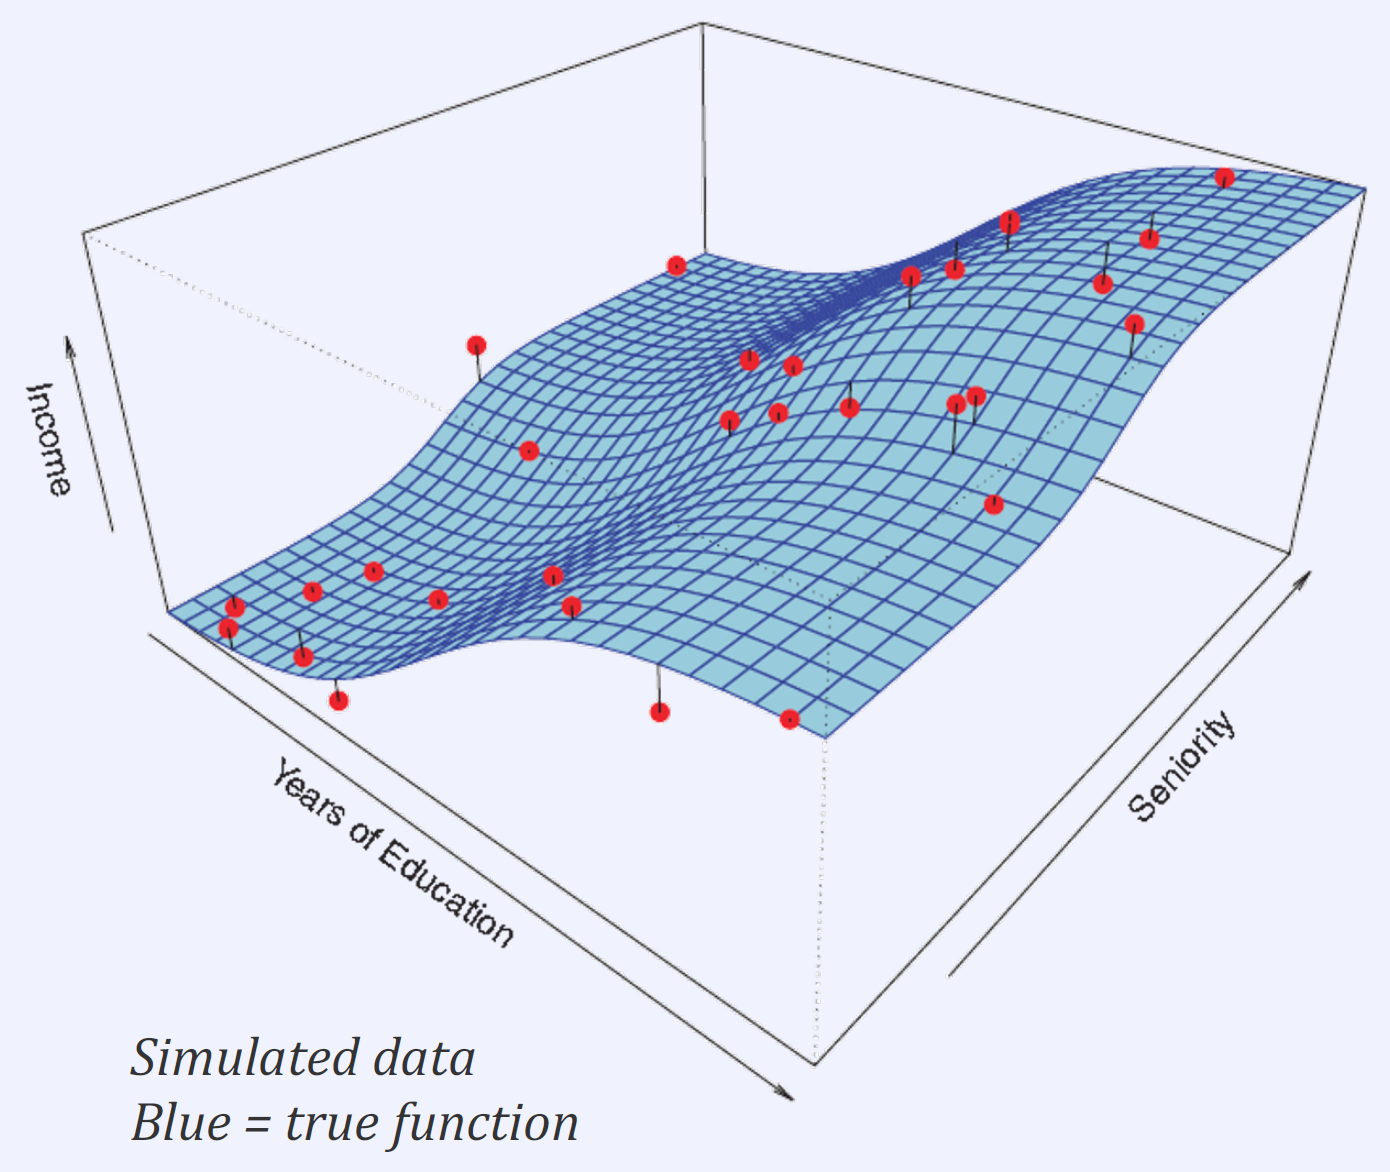
\includegraphics[width=0.3\linewidth]{Graphics/Introduction/1.png}}
			  \qquad
			  \subfloat[][]{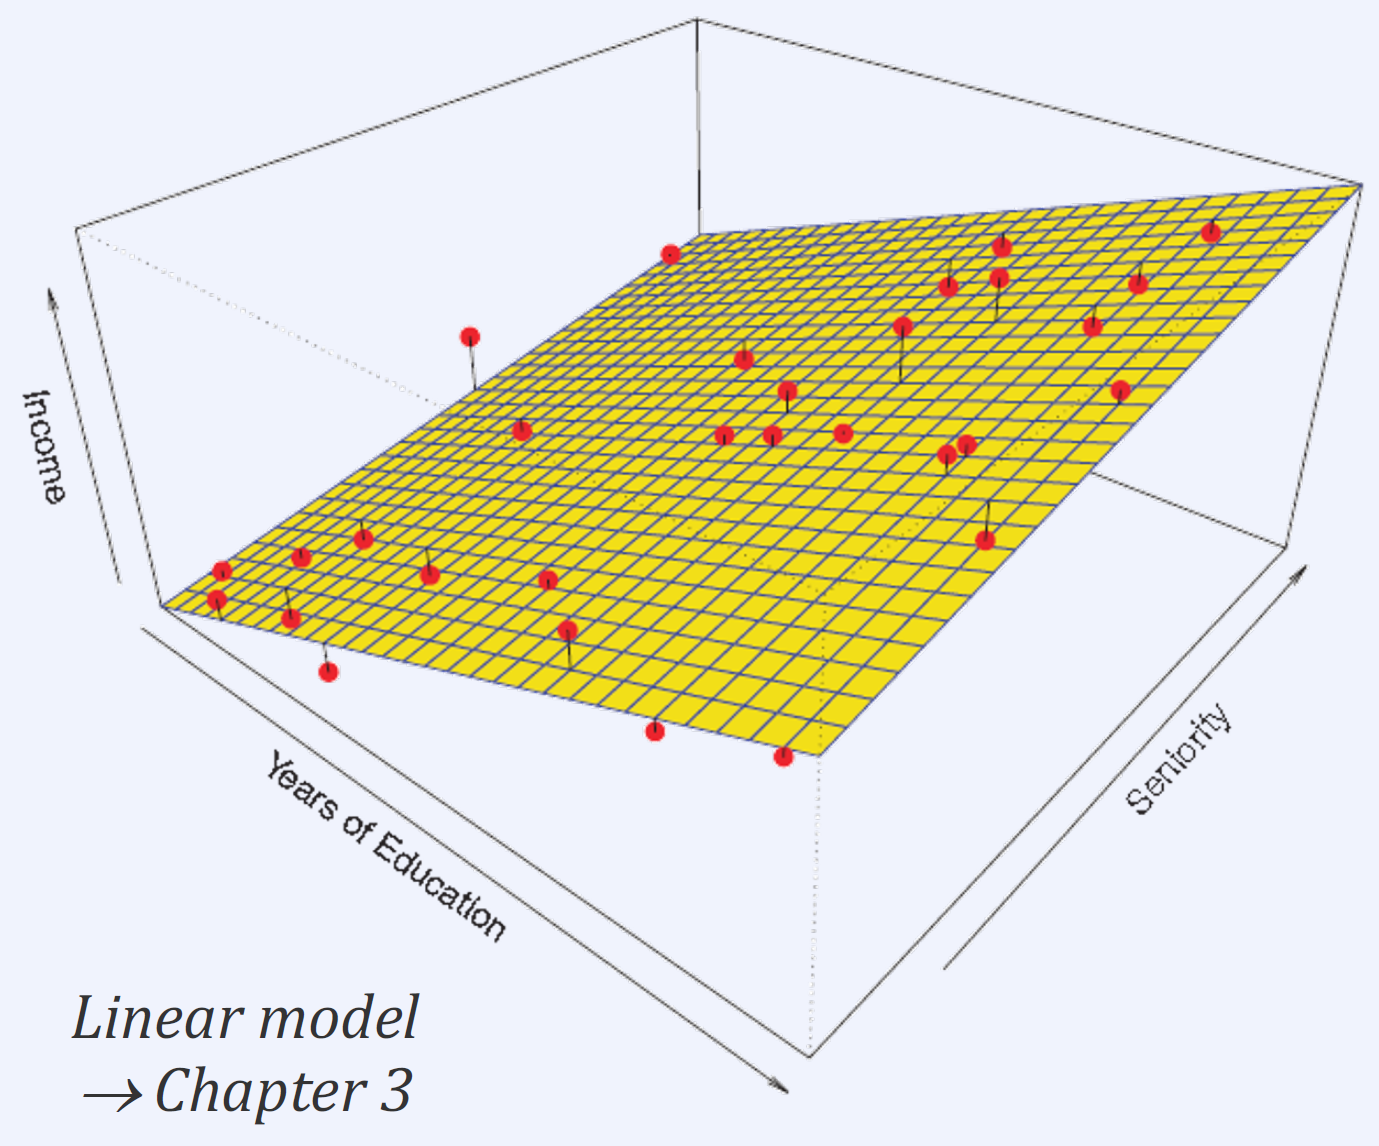
\includegraphics[width=0.3\linewidth]{Graphics/Introduction/2.png}}
			  \qquad
			  \subfloat[][]{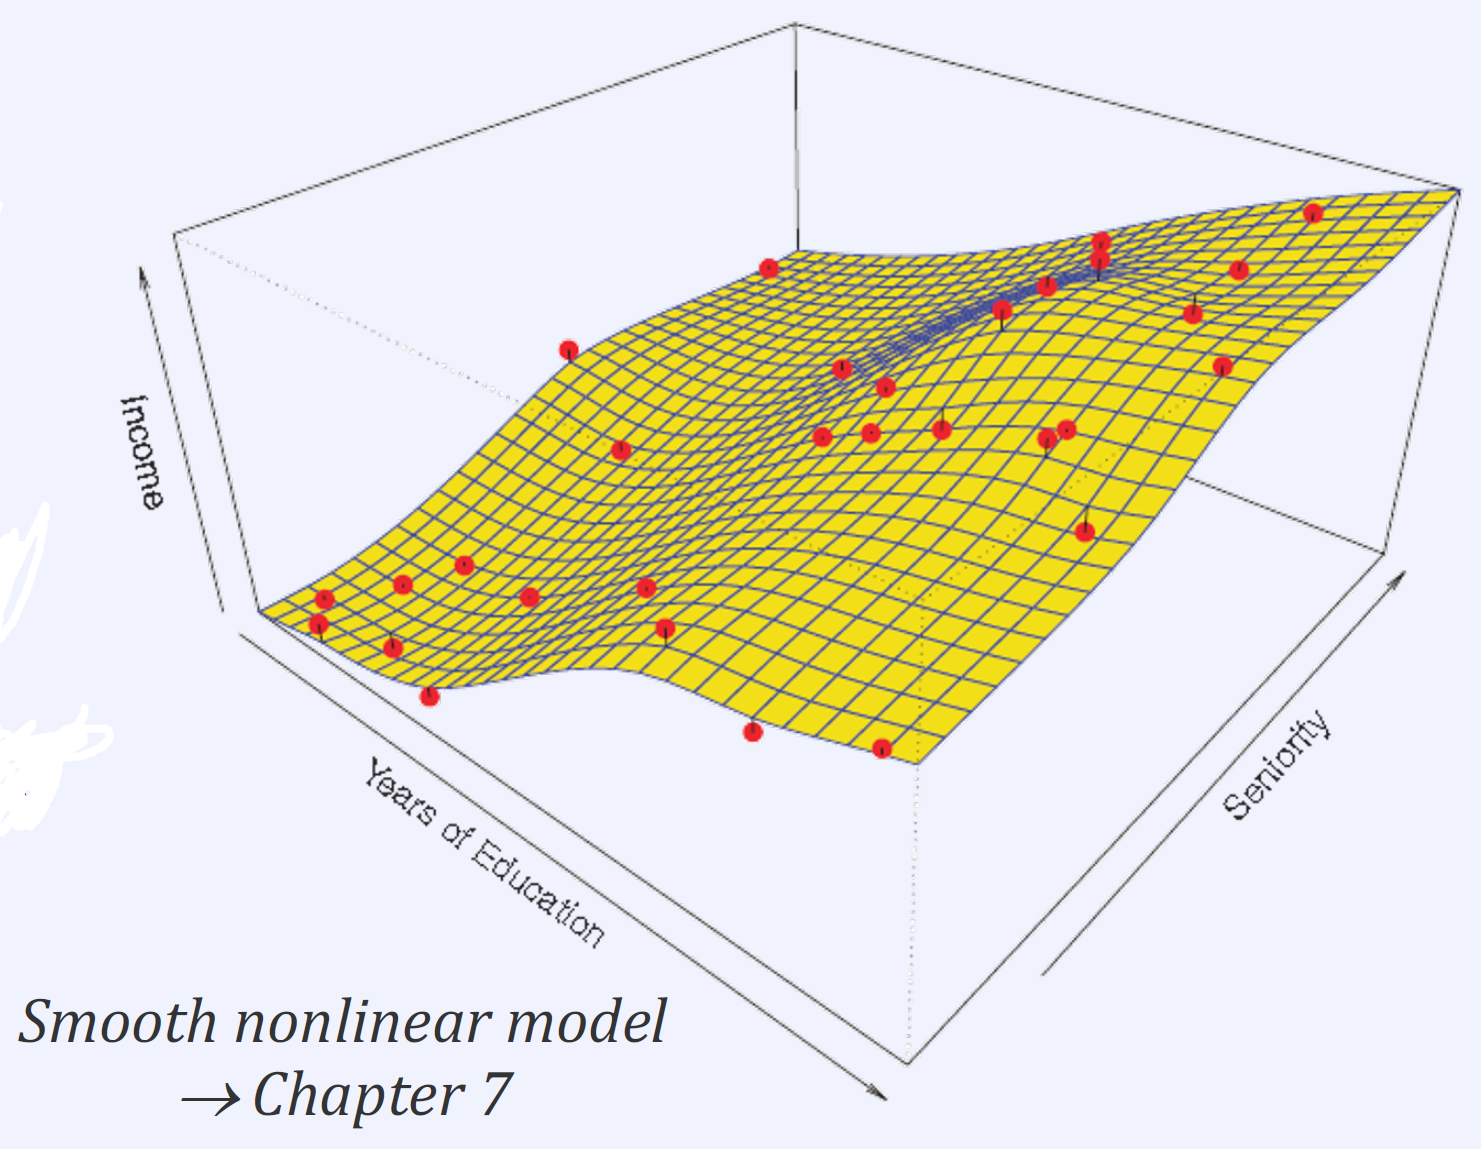
\includegraphics[width=0.3\linewidth]{Graphics/Introduction/3.png}}
			\end{figure}
	
	\section{Accuracy vs. Interpretability}
		Why would we ever prefer a more restricted model over a more flexible one?\\\\
		A flexible model entails a large number of parameters
		\begin{enumerate}
			\item Estimating all parameters is computationally expensive.
			\item Complicated models are hard to interpret, so especially when inference is the goal, simple models are preferred.
			\item If we have only few observations, we do not have enough information to accurately estimate many parameters.
			In such cases flexible models incur a high risk of overtraining.
		\end{enumerate}
	
	\section{Supervised vs. Unsupervised Learning}
		\subsection{Supervised Learning}
			\begin{itemize}
				\item \textbf{Data:} inputs and outputs $(x_i,y_i)$ for observations $i=1,...,n$ following some unknown functional pattern with noise, e.g. $Y=f(X)+\epsilon$
				\item \textbf{Goal:} find function $\hat{f}$ such that $Y \approx \hat{f}(X)$ for every conceivably seen input $X$\\
					(setting is like that of a student who learns from a teacher (supervisor) giving examples)
			\end{itemize}
		
		\subsection{Semi-supervised Learning}
			\begin{itemize}
				\item \textbf{Data:} inputs $x_i$ for observations $i=1,...,n$, only some outputs $y_i$
				\item \textbf{Goal:} same as for supervised learning, but also leverages unlabeled data
			\end{itemize}

		\subsection{Unsupervised Learning}
			\begin{itemize}
				\item \textbf{Data:} inputs $x_i$ for observations $i=1,...,n$, no outputs
				\item \textbf{Goal:} elucidate relationships between the variables or the observations\\
					(often equated with cluster analysis, but many more aspects exist)
			\end{itemize}

	\section{Assessing model accuracy}
		In regression problems we use the \textbf{mean squared error} to assass the quality of fit, here over the training data
		\begin{center}
			$MSE = \frac{1}{n} \sum\limits_{i=1}^n (y_i - \hat{f}(x_i))^2$
		\end{center}
		We call this the \textbf{training error}.\\\\
		We are more interested in the error over unseen data $(x_0,y_0)$
		\begin{center}
			$Ave(\hat{f}(x_0)-y_0)^2$
		\end{center}
		We call this the \textbf{test error}, the \textbf{generalization error}, or \textbf{expected prediction error} (EPE).\\
		If the functional dependence between input and output is not known, the test error is hard to estimate.
\newpage	
		\begin{figure}[ht]
		  \centering
		  \subfloat[][]{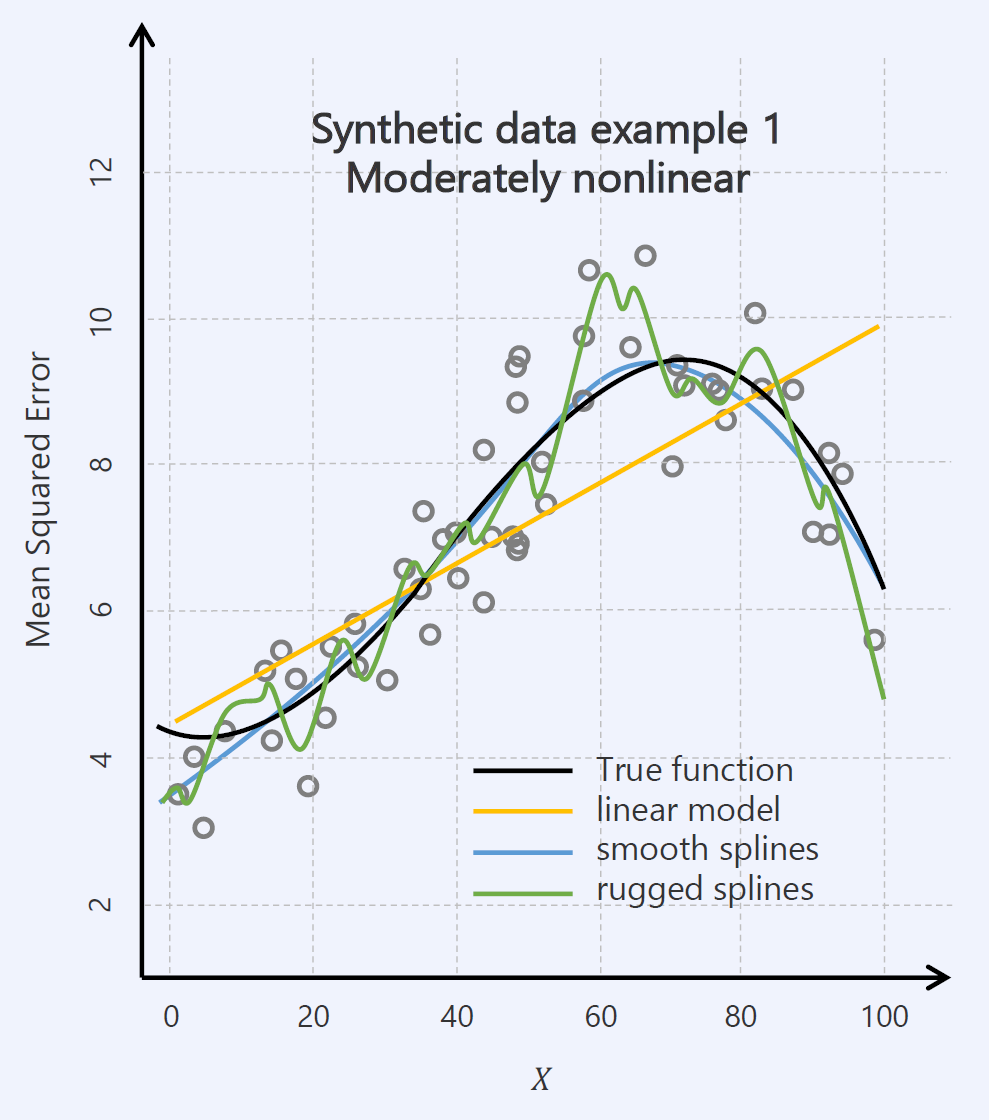
\includegraphics[width=0.33\linewidth]{Graphics/Introduction/4.png}}
		  \qquad
		  \subfloat[][]{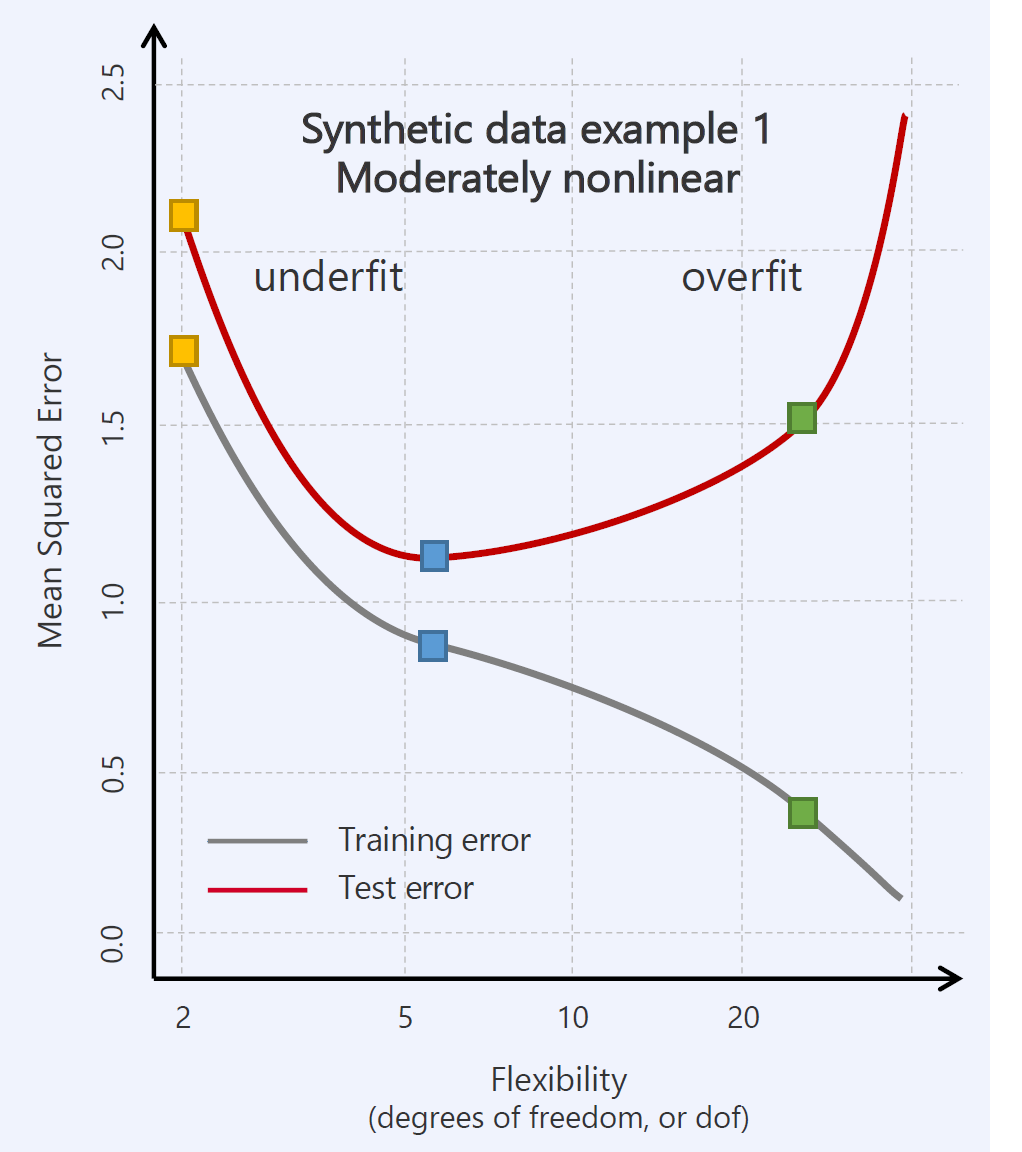
\includegraphics[width=0.33\linewidth]{Graphics/Introduction/5.png}}
		\end{figure}
		\begin{figure}[ht]
		  \centering
		  \subfloat[][]{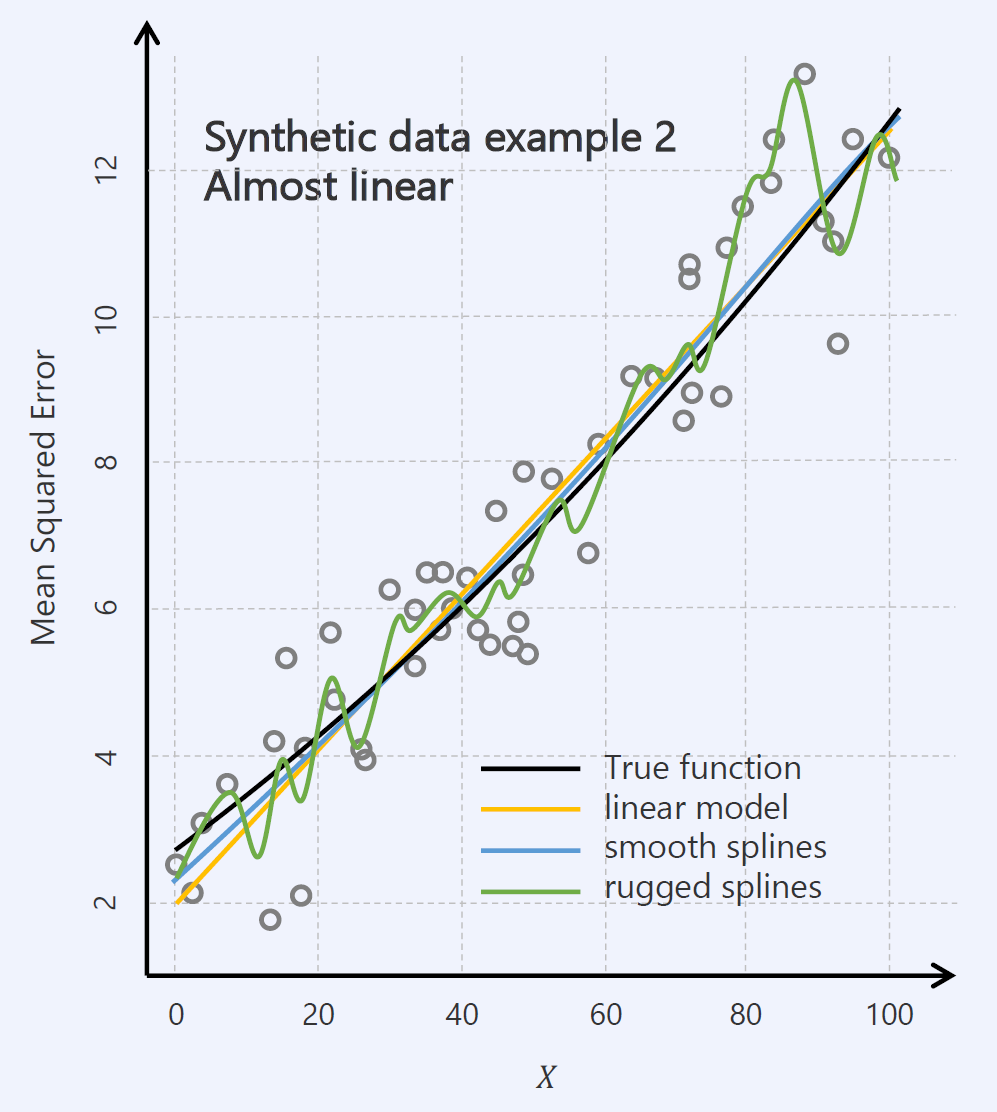
\includegraphics[width=0.33\linewidth]{Graphics/Introduction/6.png}}
		  \qquad
		  \subfloat[][]{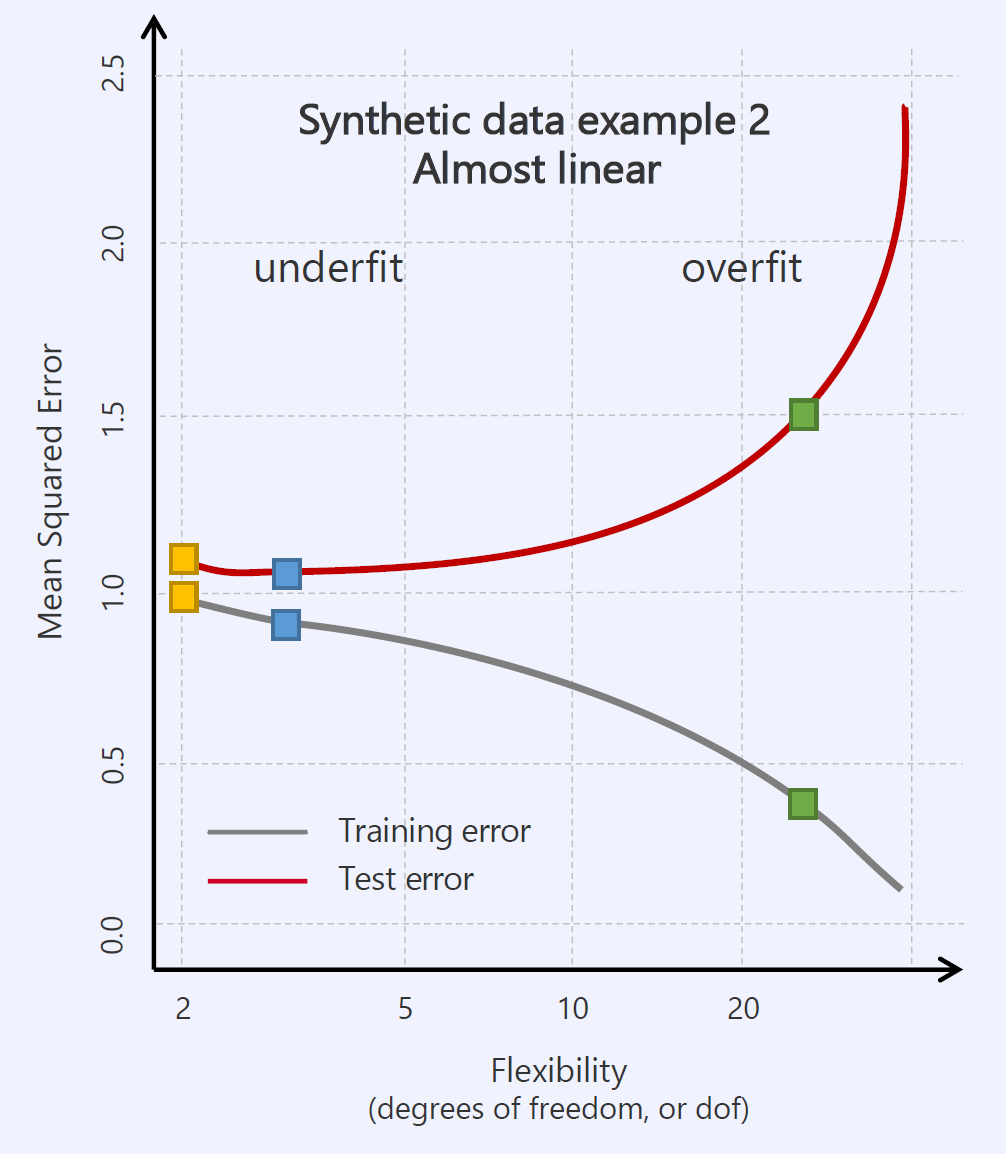
\includegraphics[width=0.33\linewidth]{Graphics/Introduction/7.png}}
		\end{figure}
		\begin{figure}[ht]
		  \centering
		  \subfloat[][]{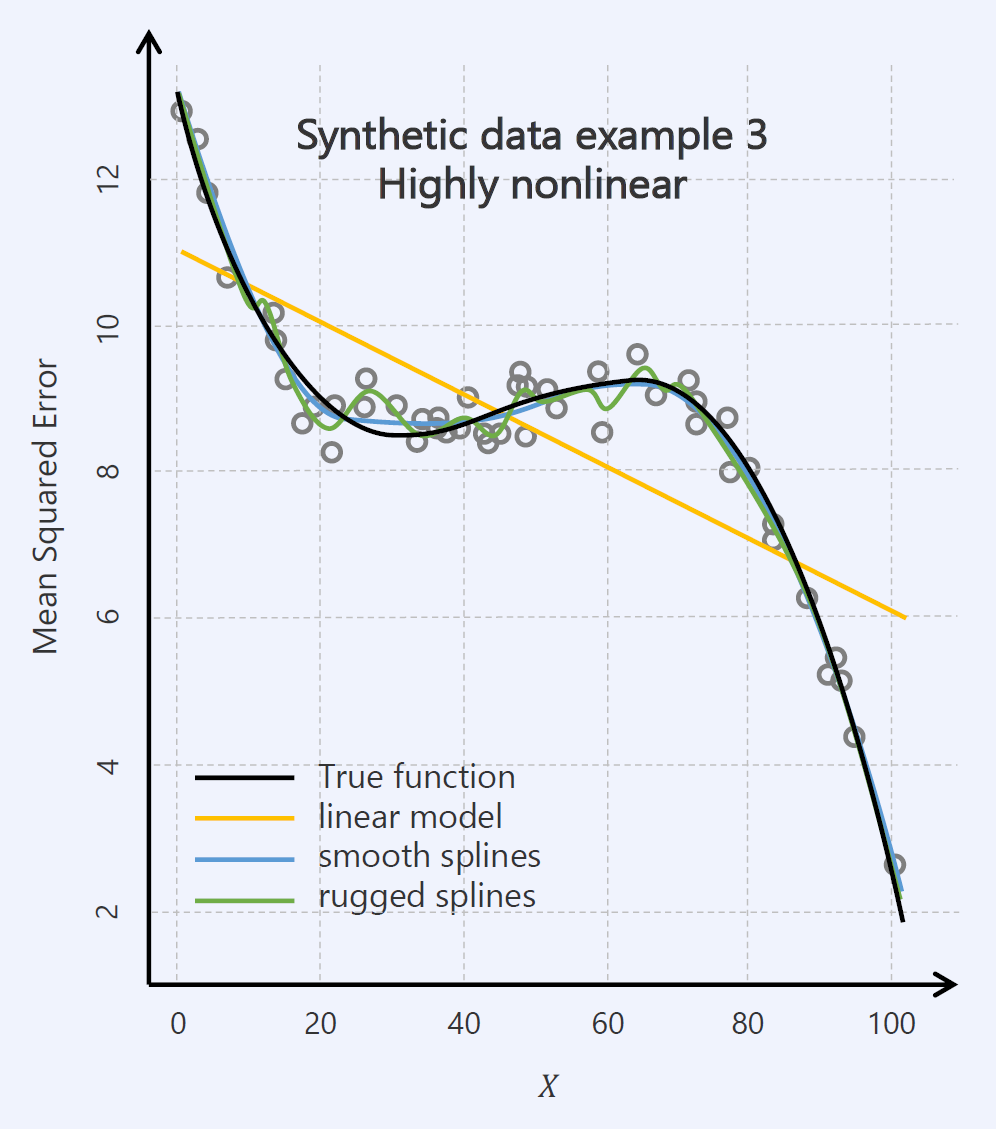
\includegraphics[width=0.33\linewidth]{Graphics/Introduction/8.png}}
		  \qquad
		  \subfloat[][]{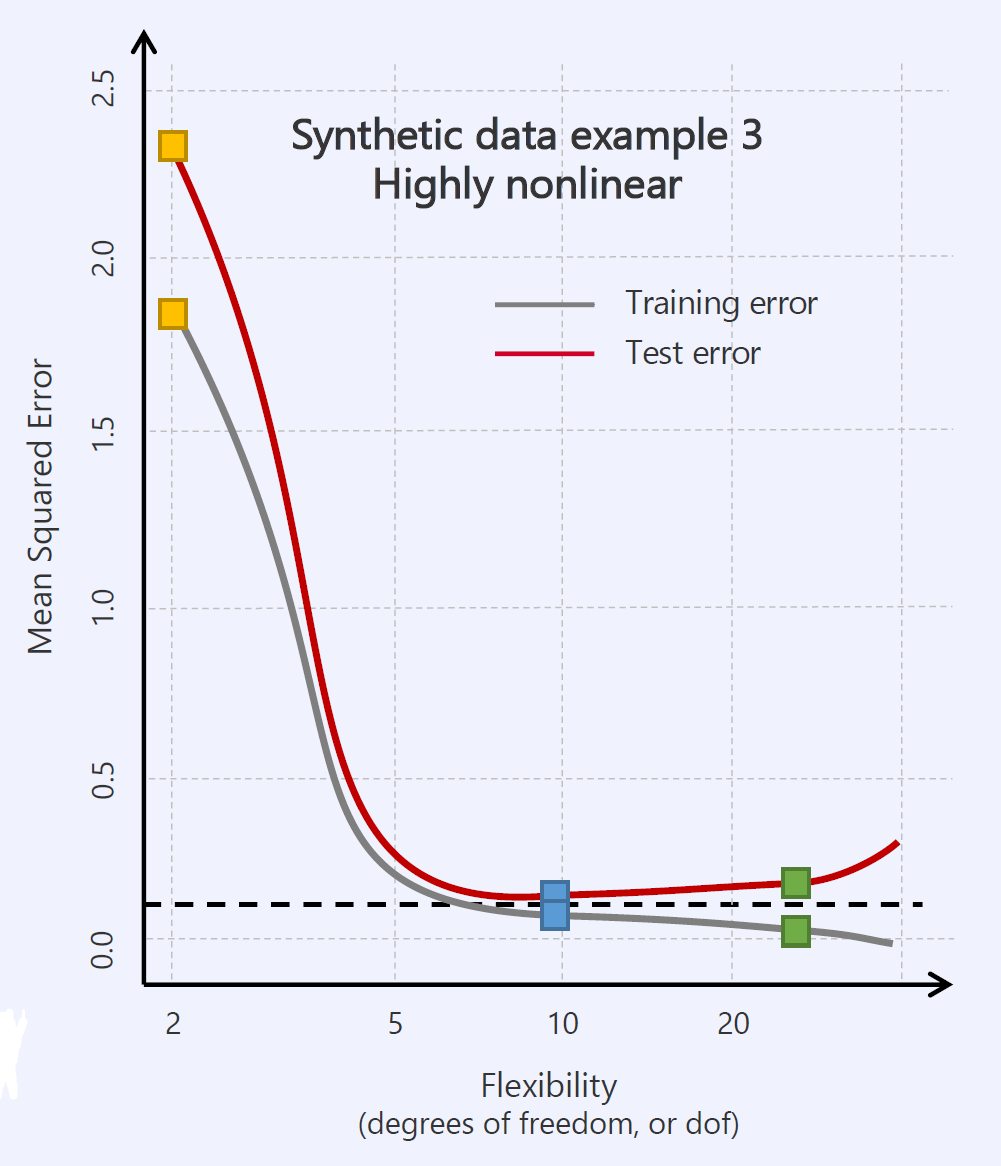
\includegraphics[width=0.33\linewidth]{Graphics/Introduction/9.png}}
		\end{figure}
\newpage

	\section{Bias-Variance}
		\subsection{Tradeoff}
			The shape of the curve for test error is due to a basic tradeoff in the $MSE$
			\begin{center}
				$E[y_0-\hat{f}(x_0)]^2 = Var(\hat{f}(x_0)) + [Bias(\hat{f}(x_0))]^2 + Var(\epsilon)$
			\end{center}
			Here \textbf{bias} is the systematic deviation of the estimate from the true value
			\begin{center}
				$Bias(\hat{f}(x_0)) = E[\hat{f}(x_0)-y_0]$
			\end{center}
			and \textbf{variance} is the variation of the estimate between different training sets
			\begin{center}
				$Var(\hat{f}(x_0)) = E[\hat{f}(x_0)-E[\hat{f}(x_0)]]^2$
			\end{center}

		\subsection{Bias-Variance Decomposition}
			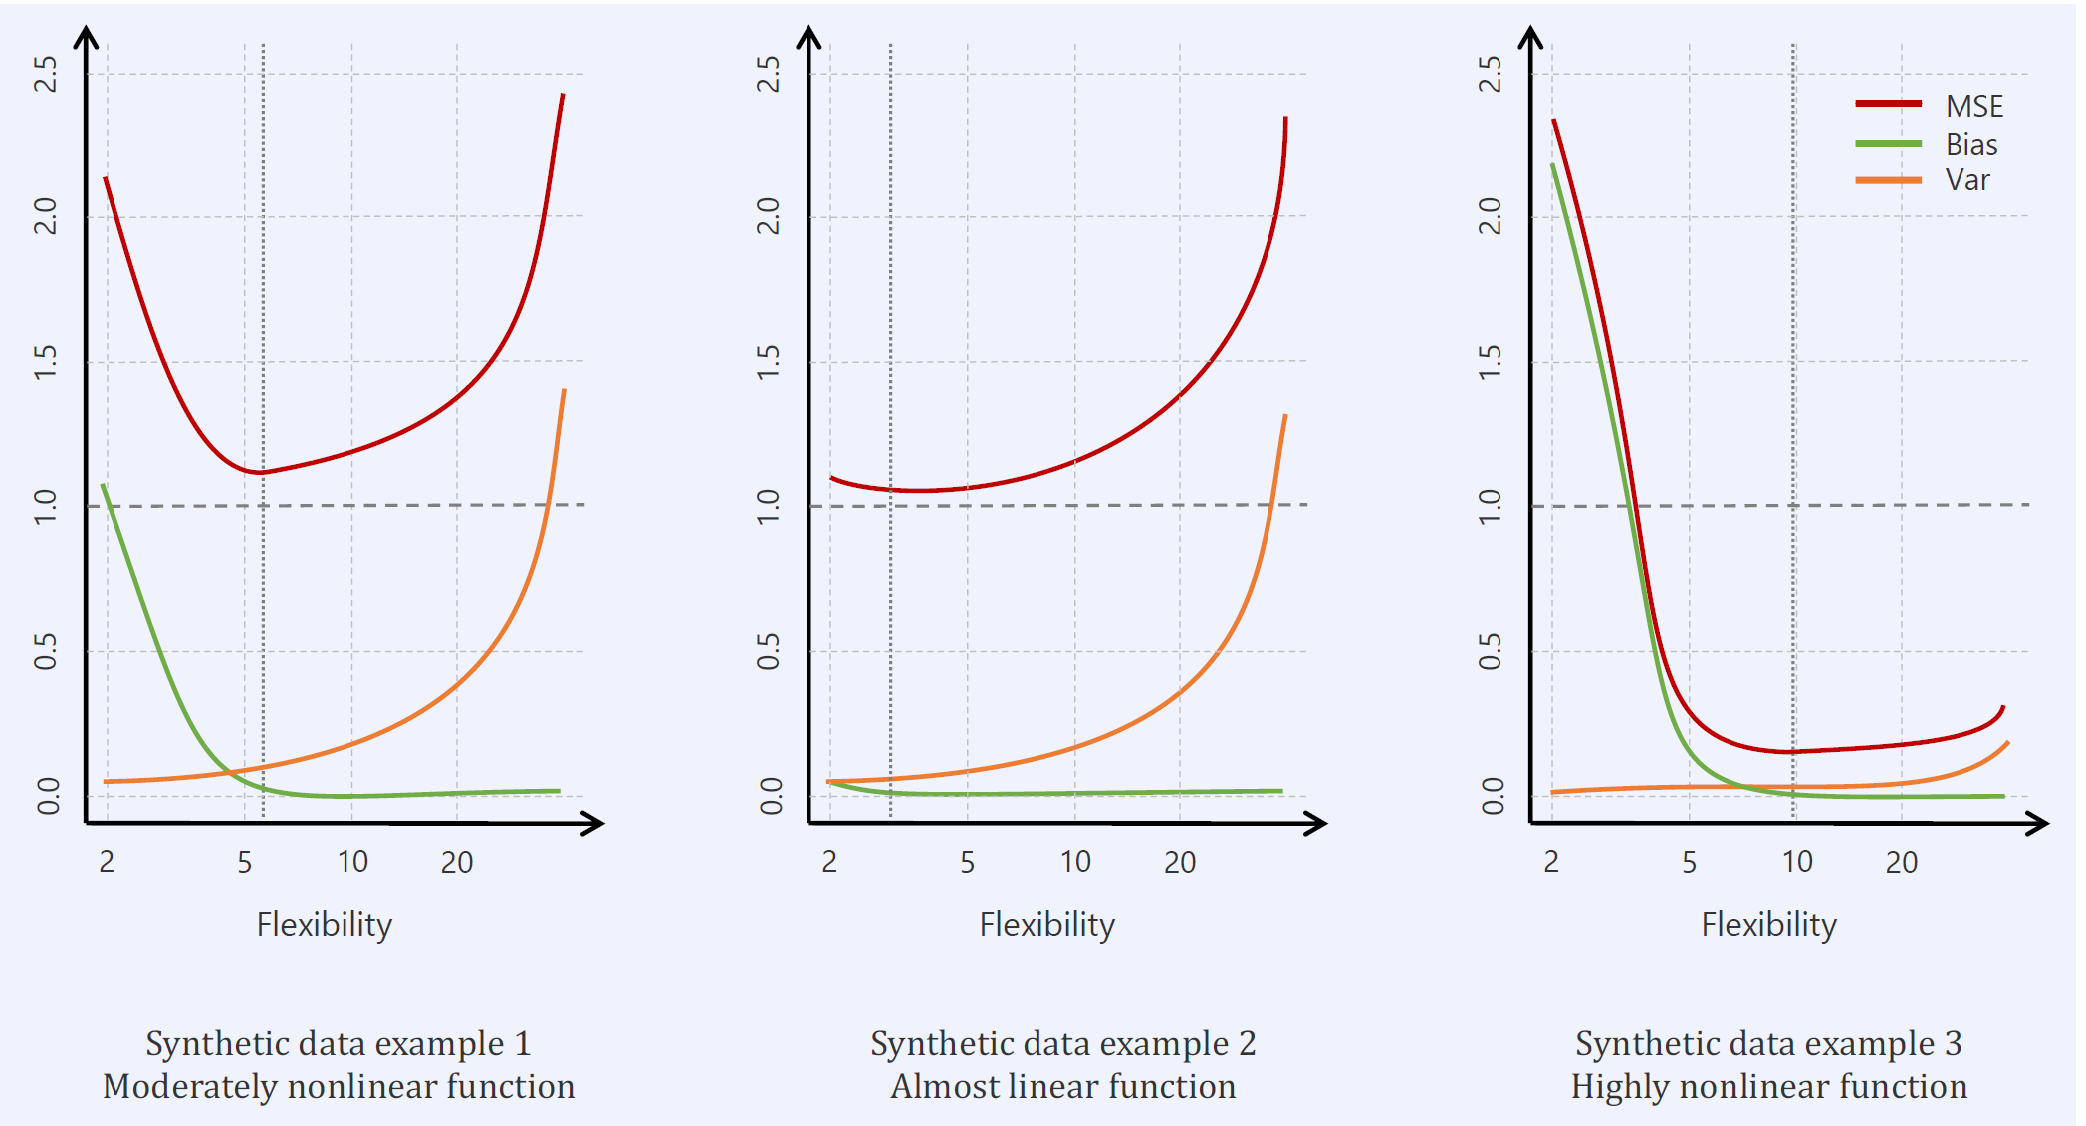
\includegraphics[width=1.05\linewidth]{Graphics/Introduction/10.png}
	
	\section{The Classification Setting}
		A popular method of measuring classification error (\textbf{loss function}) is the \textbf{misclassification error}.\\\\
		On the training set is
		\begin{center}
			$\frac{1}{n} \sum\limits_{i=1}^n I(y_i \neq \hat{y}_i)$
		\end{center}
		where for a predicate $p$,
		\begin{itemize}
			\item $I(p)=1$ if $p=true$ and
			\item $I(p)=0$ otherwise.
		\end{itemize}
		The test error is
		\begin{center}
			$AVE(I(y_0 \neq \hat{y}_0))$
		\end{center}
		
		\subsection{Bayes Classifier}
			The test error is minimized by the following very simple calssifier
			\begin{center}
				$arg \underset{j=1,...,k}{max} Pr[Y=j \mid X=x_0]$
			\end{center}
			for a classification problem with $k$ classes $1,...,k$.\\\\
			This classifier can be computed on \textbf{synthetic data} for which the \textbf{probability distribution is known}, but not for real data, 
			as we do not know the probability distribution.

	\section{Example Binary Classification}
			100 observations in each of two groups, synthetic data with noise.
			\begin{itemize}
				\item \textbf{Bayes decision boundary:} points with $Pr[Y=1 \mid X=x_0] = 0.5$ is dashed.
				\item \textbf{Bayes error rate:} the irreducible error $1 - E[\underset{j=1,2}{max} Pr[Y=j \mid X]]$ in genaral, and $0.1304$ for this example.
			\end{itemize}
			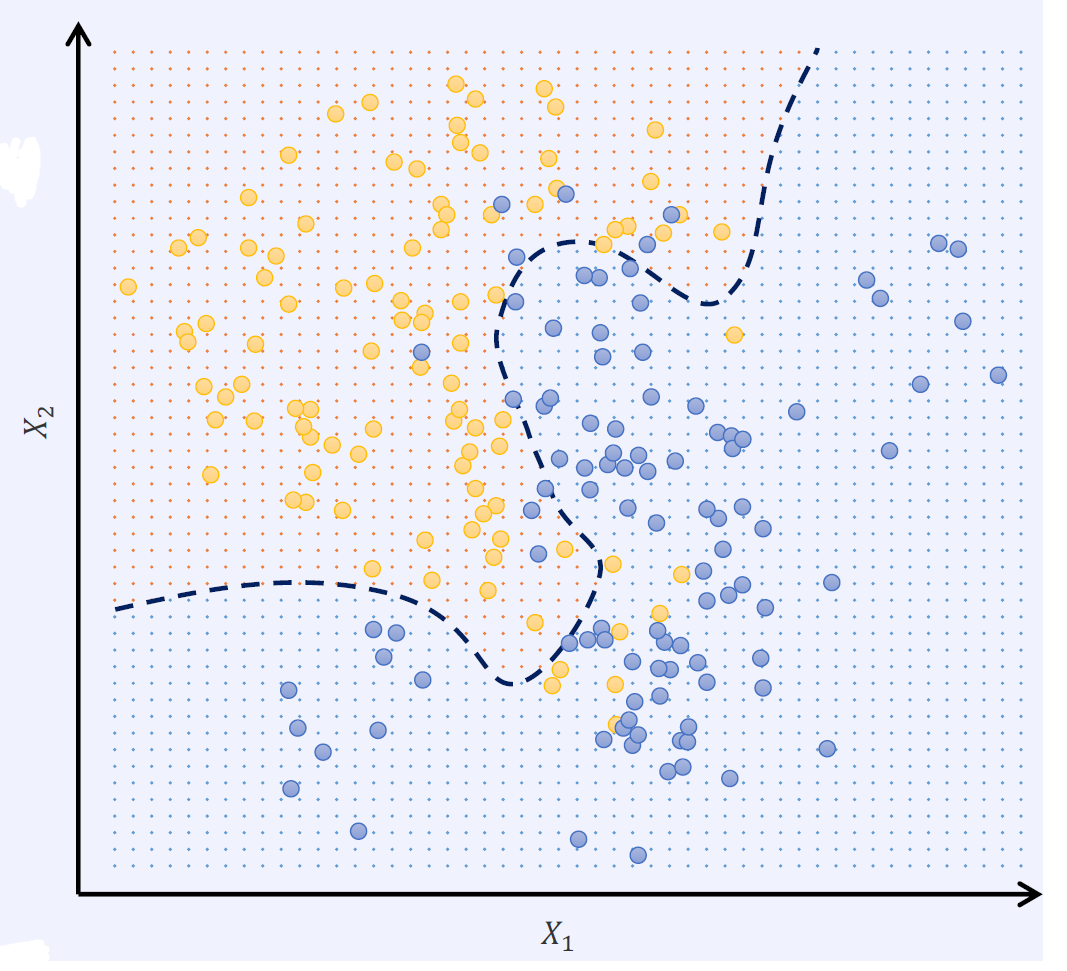
\includegraphics[width=1\linewidth]{Graphics/Introduction/11.png}
\newpage		
		\subsection{Nearest Neighbors}
			\textbf{$k$-nearest neighbors ($k$NN)}\\
			Classifies each pointto the majority class among its $k$ nearest neighbors
			\begin{center}
				$arg \underset{j=1,...,k}{max} \frac{1}{k} \sum\limits_{\mathbb{N}_0} I(y_i = j)$
			\end{center}
			where $\mathbb{N}_0$ is the set of the $k$ data points nearest to $x_0$.
			
			\begin{figure}[ht]
			  \centering
			  \subfloat[][]{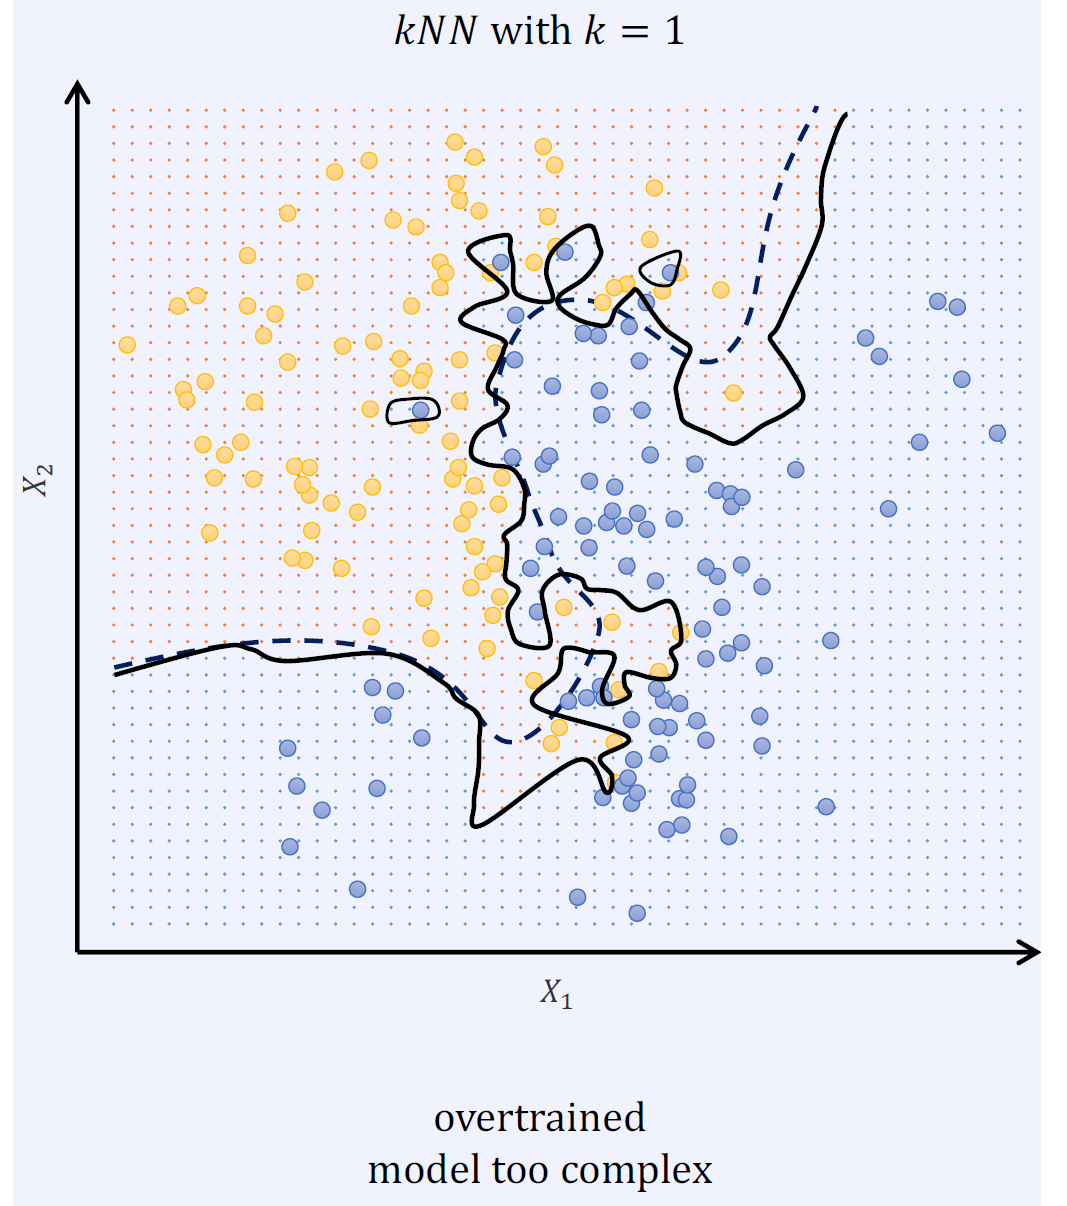
\includegraphics[width=0.3\linewidth]{Graphics/Introduction/12.png}}
			  \qquad
			  \subfloat[][]{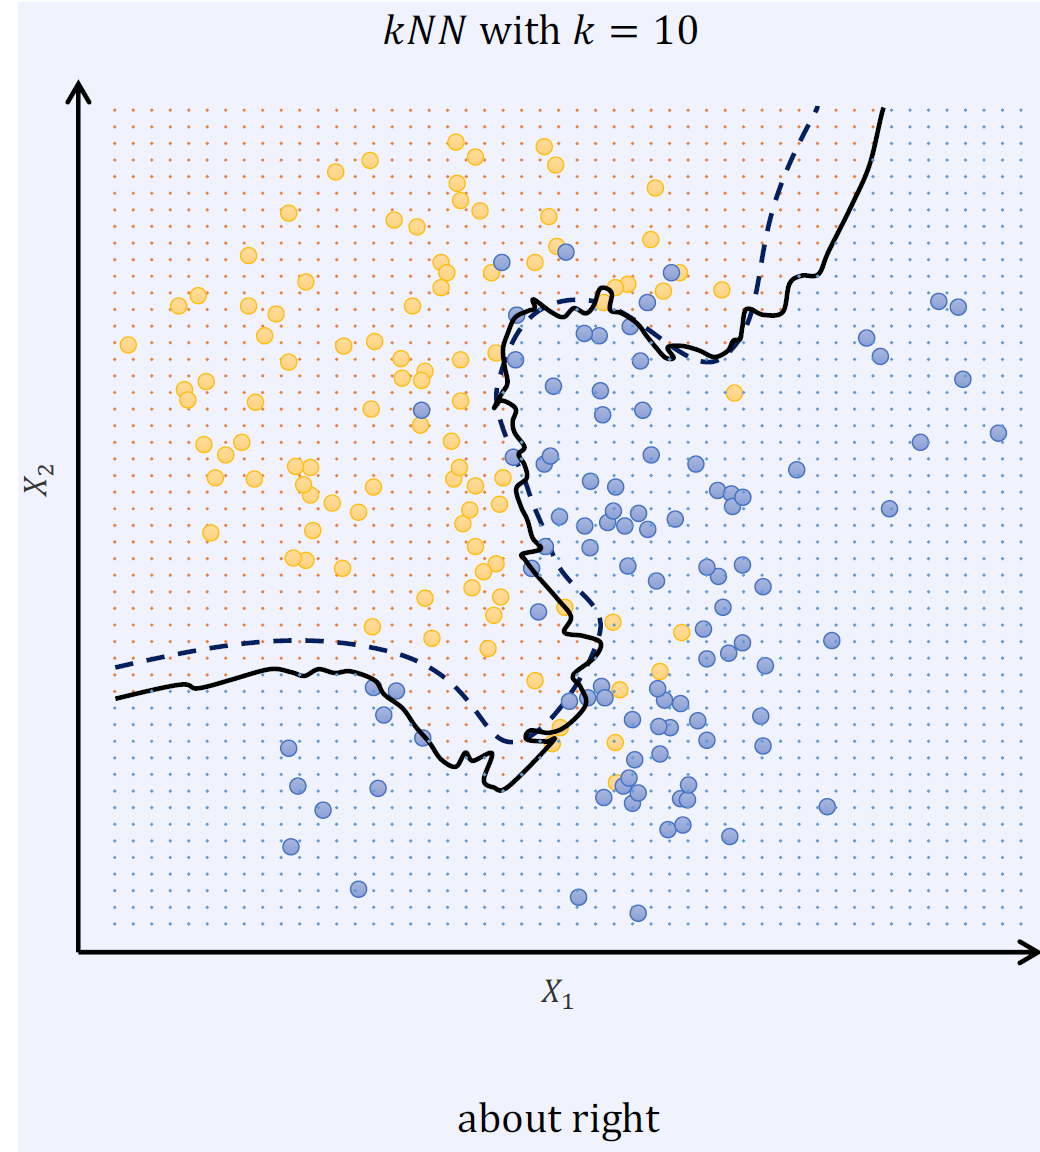
\includegraphics[width=0.3\linewidth]{Graphics/Introduction/13.png}}
			  \qquad
			  \subfloat[][]{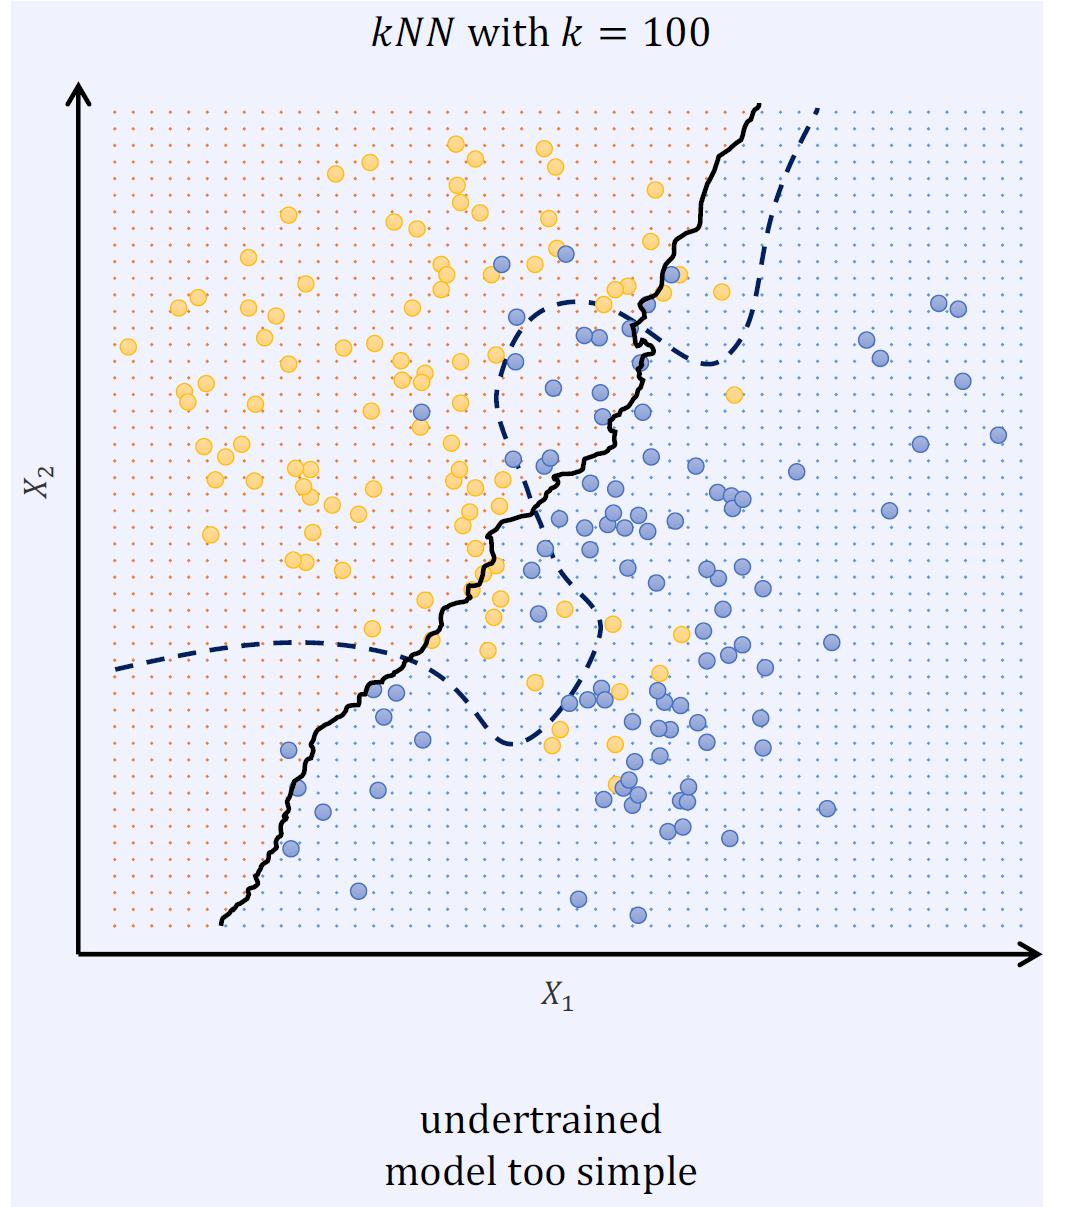
\includegraphics[width=0.3\linewidth]{Graphics/Introduction/14.png}}
			\end{figure}

			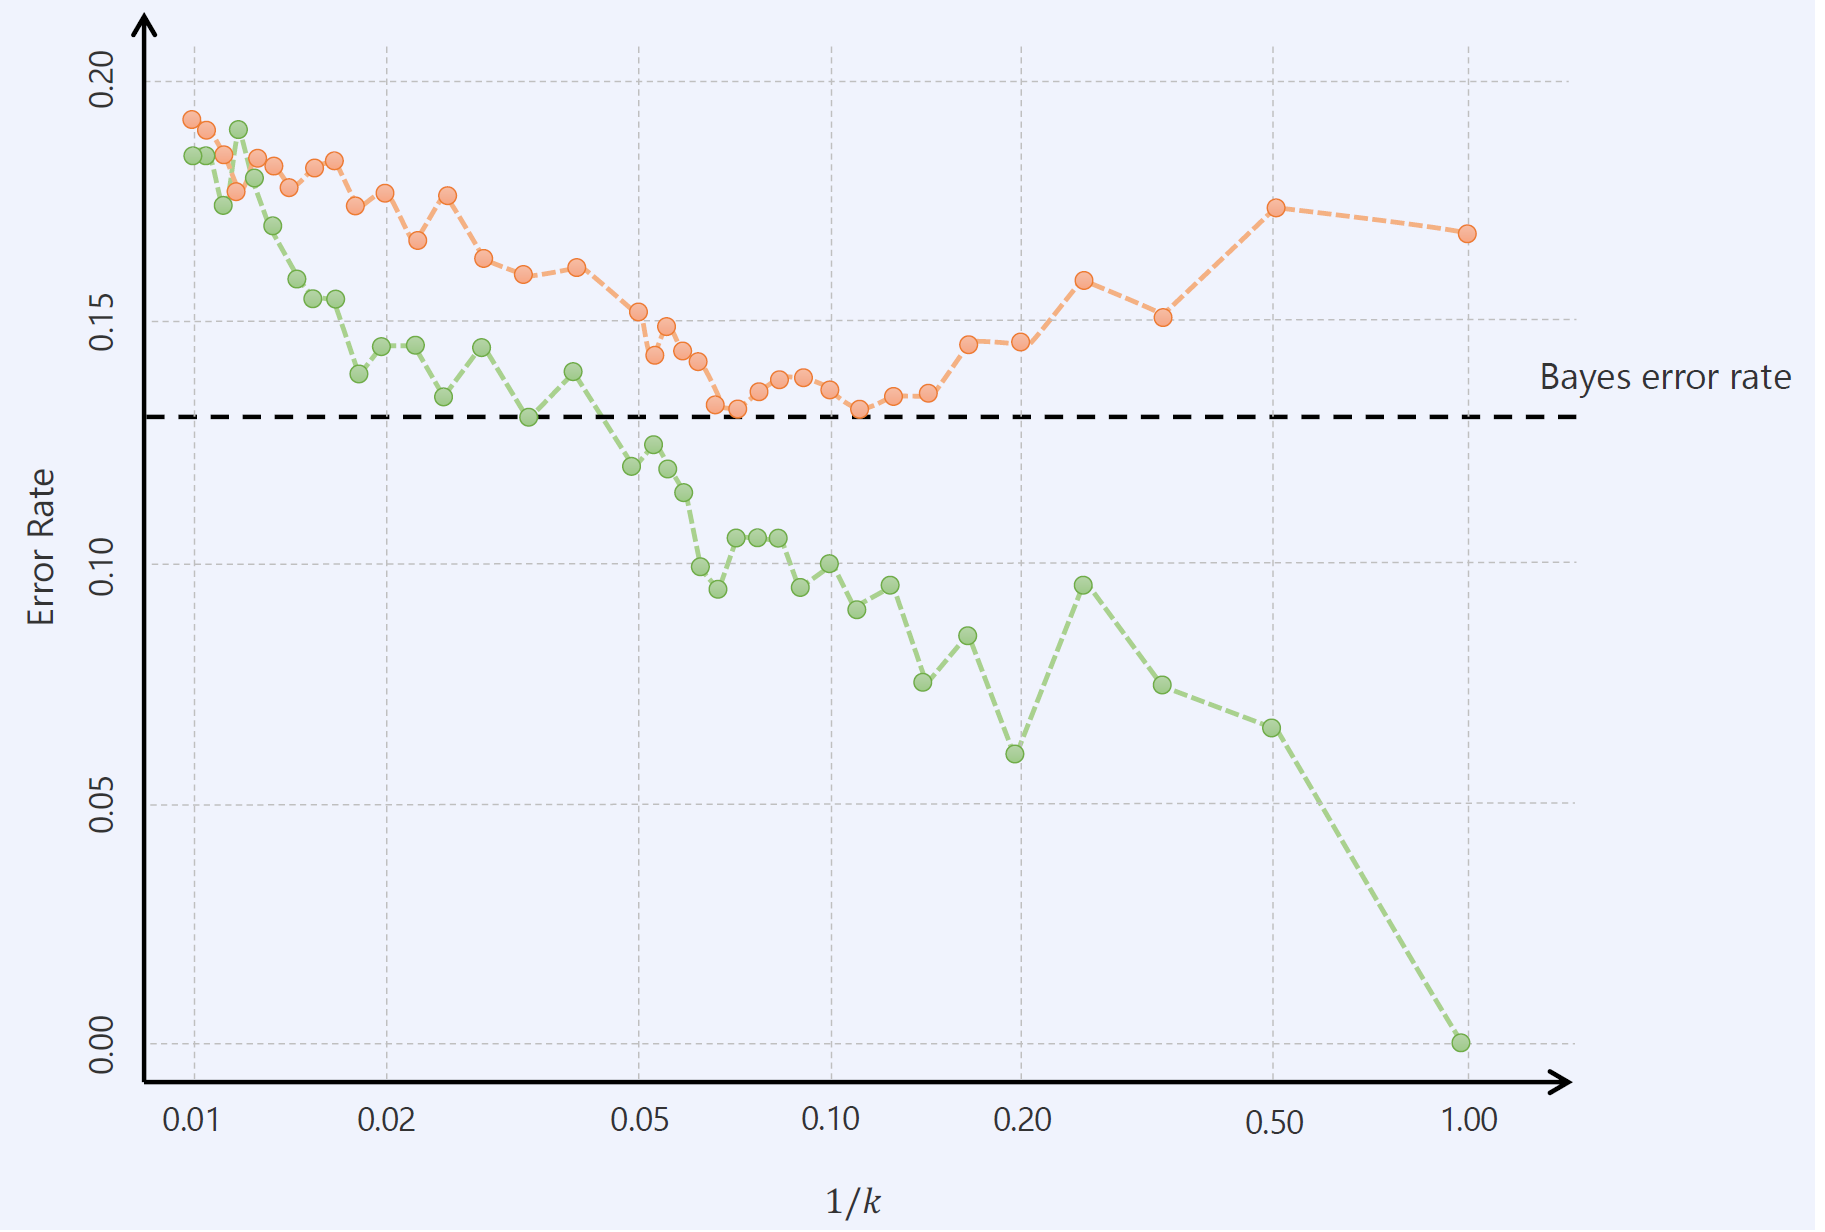
\includegraphics[width=1\linewidth]{Graphics/Introduction/15.png}
































\end{document}
